\documentclass[aspectratio=169,11pt]{beamer}

\usepackage[T1]{fontenc}
\usepackage{lmodern}
\usepackage{booktabs}
\usepackage{array}
\usepackage{algorithm}
\usepackage{algpseudocode}
\usepackage{tikz}
\usetikzlibrary{positioning,arrows.meta}

% Simple, standard look
\usetheme{default}
\definecolor{accent}{HTML}{1F5F5B}
\definecolor{warn}{HTML}{A8502A}
\definecolor{grey}{HTML}{5C6670}
\definecolor{soft}{HTML}{E3EFED}
\setbeamercolor{structure}{fg=accent}
\setbeamercolor{frametitle}{fg=accent}
\setbeamercolor{title}{fg=accent}
\setbeamerfont{frametitle}{series=\bfseries}
\setbeamerfont{title}{series=\bfseries,size=\LARGE}
\setbeamertemplate{navigation symbols}{}
\setbeamertemplate{footline}[frame number]
\setbeamertemplate{itemize items}[circle]
\renewcommand{\arraystretch}{1.3}
\newcolumntype{L}[1]{>{\raggedright\arraybackslash}p{#1}}
\newcolumntype{C}[1]{>{\centering\arraybackslash}p{#1}}

\newcommand{\yes}[1]{\textcolor{accent}{\textbf{#1}}}
\newcommand{\no}[1]{\textcolor{warn}{\textbf{#1}}}
\newcommand{\h}[1]{\textcolor{grey}{#1}}
\newcommand{\remark}[1]{\par\vspace{0.35cm}{\small\textcolor{grey}{#1}}}
\algrenewcommand\algorithmicrequire{\textbf{Input:}}
\algrenewcommand\algorithmicensure{\textbf{Output:}}

\title{Multi-Agent Systems for Image Analysis:\\Object and Complex Scene Detection}
\subtitle{Cross-Modal Agent Disagreement as a Bounded Signal for Epistemic Uncertainty in Low-Fidelity Historical Scans}
\author{Brhanu Atsbaha}
\date{2 October 2026\\[6pt]
\small First advisor: Prof.\ Dr.\ Thomas Mandl \quad Second advisor: Shereen Elsayed}

\begin{document}

\begin{frame}[plain]
  \titlepage
\end{frame}

% ========================================================================
\begin{frame}{Outline}
\begin{enumerate}\setlength\itemsep{6pt}
  \item The goal and the data
  \item Since 14 September: what changed, and what you asked for
  \item How the system works: architecture and algorithms
  \item What was wrong with the old design, and what we changed
  \item Results: accuracy, automatic approval, the risk promise
  \item The main research question, and human agreement
  \item What is still open, and the decisions we need
\end{enumerate}
\end{frame}

% ========================================================================
\begin{frame}{The goal}
The Colibri archive holds \textbf{thousands of pictures} from historical children's books. Describing them by hand is too slow, so programs (agents) describe them automatically. But the programs make mistakes.
\vspace{0.3cm}
\begin{itemize}\setlength\itemsep{8pt}
  \item For every picture the system decides: \textbf{accept the answer}, or \textbf{send it to a person}.
  \item It gives a promise in advance: of the accepted answers, \textbf{at most 5 in 100} are wrong.
  \item Main question (RQ1): does \textbf{disagreement} between the agents warn us of mistakes?\\
        Answer: \textbf{no}. The system's own \textbf{confidence} warns better.
\end{itemize}
\remark{The contribution is not a better detector; it is knowing which answers can be trusted.}
\end{frame}

% ========================================================================
\begin{frame}{The data}
\begin{tabular}{@{}L{4.2cm} L{8.6cm}@{}}
\toprule
\h{Set} & \h{What it is and what it is used for}\\
\midrule
Whole archive & All pictures; every model runs on all of them\\
The 300 & Pictures a person labelled object by object: the answer key for objects\\
The scene pool & 1,250 pictures with a checked scene label, from 550 books\\
\quad practice (train) & 749: the system learns its translation rules here\\
\quad calibration & 252: the risk cut-off is chosen here\\
\quad test & 249: used only to measure, never to tune\\
\bottomrule
\end{tabular}
\end{frame}

% ========================================================================
\begin{frame}{Since 14 September: then and now}
\begin{tabular}{@{}L{2.8cm} L{4.6cm} L{5.4cm}@{}}
\toprule
 & \h{14 September} & \h{Now}\\
\midrule
The agents     & Signals not what their names said & Corrected: wrong answers 25.4\% $\to$ 15.6\%\\
Disagreement   & Does not warn of mistakes         & Re-tested per class: still no\\
The promise    & Holds, on old signals             & Holds; 15.8 points more approved\\
Inputs         & Partly old stored signals         & Everything rerun from the pictures\\
Object finder  & Weak                              & Retrained: 0.123 $\to$ 0.205\\
Test pictures  & 38 without a scene                & 65 without a scene (target 80)\\
\bottomrule
\end{tabular}
\remark{On 14 September the thesis was mainly a careful negative result. It now also has a proven positive result.}
\end{frame}

% ========================================================================
\begin{frame}{What you asked for on 14 September}
\small
\begin{tabular}{@{}L{5.6cm} L{1.9cm} L{5.2cm}@{}}
\toprule
\h{Request} & \h{Status} & \h{Result}\\
\midrule
Each model and the fusion on the 300 & \yes{done} & Describer best (F1 0.65)\\
Other models' view of the pseudo-labels & \yes{done} & 71--100\% confirmed\\
20 pseudo-labels checked by hand & \no{19 of 20} & All well placed\\
Which classes get detected & \yes{done} & 126 of 128 misses were the teacher's\\
A better student--teacher setup & \yes{done} & 0.123 $\to$ 0.205\\
Agreement per class, with kappa & \yes{done} & Objects and scene types\\
Find rare objects & \no{prepared} & 548 pictures ready to label\\
Is disagreement what we need? & \yes{answered} & No\\
\bottomrule
\end{tabular}
\remark{The text reader is out, so there are 3 models and 3 pairs per class, not 4 and 6.}
\end{frame}

% ========================================================================
\begin{frame}{Each model on the 300 hand-labelled pictures}
\begin{columns}[T]
\column{0.5\textwidth}
\begin{tabular}{@{}l c c@{}}
\toprule
\h{Model (mean of 8 classes)} & \h{Ranking} & \h{F1}\\
\midrule
\textbf{Describer (LLaVA)} & \textbf{0.91} & \textbf{0.65}\\
All three combined & 0.90 & 0.60\\
Scene matcher (SigLIP) & 0.85 & 0.51\\
Old object finder & 0.62 & 0.35\\
Text reader, text class only & 0.55 & 0.38\\
Always answering ``yes'' & -- & 0.28\\
\bottomrule
\end{tabular}
\column{0.46\textwidth}\small
\begin{itemize}\setlength\itemsep{6pt}
  \item \textbf{Describer:} best on every class once asked one yes/no question per class.
  \item \textbf{Old object finder:} good for person (F1 0.80) and animal (0.70) only; never finds text.
  \item \textbf{Scene matcher:} ranks well, but its raw scores need calibrating.
  \item Blurry prints are not harder (describer 0.66 vs 0.65).
\end{itemize}
\end{columns}
\remark{Ranking = AUROC (0.5 coin flip, 1 perfect). Cut-offs chosen by 5-fold cross-validation.}
\end{frame}

% ========================================================================
\begin{frame}{The teacher's labels, and a better teacher}
\begin{columns}[T]
\column{0.5\textwidth}\small
\begin{itemize}\setlength\itemsep{6pt}
  \item Other models confirm \textbf{71--100\%} of the labels the object finder learned from.
  \item On the 3,000-picture set they confirm only person 52\%, animal 18\%, child 2\%, weapon 0\%.
  \item 19 of 20 boxes checked by hand: all well placed; two class names wrong.
  \item \textbf{126 of 128} student misses were never labelled by the teacher.
\end{itemize}
\column{0.46\textwidth}\small
\begin{tabular}{@{}l c@{}}
\toprule
\h{Box accuracy (AP50)} & \h{Score}\\
\midrule
Old student & 0.123\\
\textbf{New student} & \textbf{0.205}\\
New teacher & 0.283\\
\midrule
Unseen pictures, old / new & 0.106 / 0.186\\
\bottomrule
\end{tabular}
\end{columns}
\remark{Biggest gains on classes the old teacher never labelled: building 0.05 $\to$ 0.23, vehicle 0 $\to$ 0.23, child 0.05 $\to$ 0.13.}
\end{frame}

% ========================================================================
\begin{frame}{Architecture: how the agents work together}
\centering
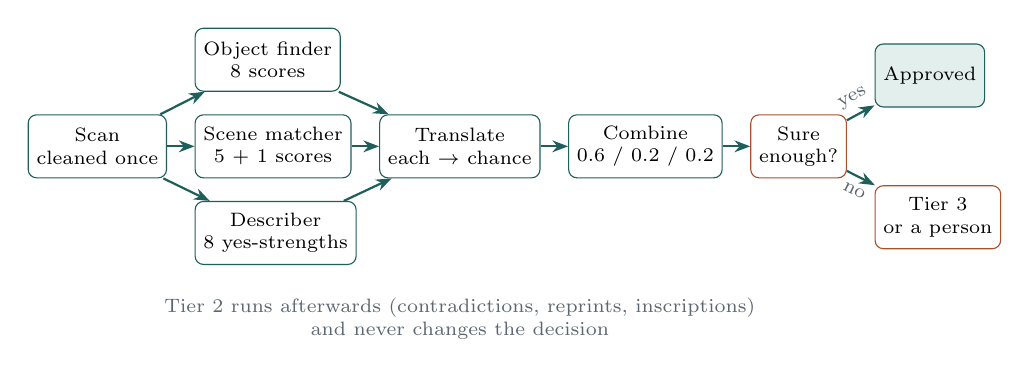
\begin{tikzpicture}[font=\scriptsize, node distance=3mm and 3.5mm,
  box/.style={draw=accent, rounded corners=3pt, align=center, minimum height=8mm, inner sep=3pt, fill=white},
  dec/.style={draw=warn, rounded corners=3pt, align=center, minimum height=8mm, inner sep=3pt, fill=white},
  arr/.style={-{Stealth[length=2mm]}, accent, thick}]
  \node[box] (scan) {Scan\\cleaned once};
  \node[box, right=of scan, yshift=11mm] (obj) {Object finder\\8 scores};
  \node[box, right=of scan] (sce) {Scene matcher\\5 + 1 scores};
  \node[box, right=of scan, yshift=-11mm] (vlm) {Describer\\8 yes-strengths};
  \node[box, right=of sce] (tr) {Translate\\each $\to$ chance};
  \node[box, right=of tr] (comb) {Combine\\0.6 / 0.2 / 0.2};
  \node[dec, right=of comb] (sure) {Sure\\enough?};
  \node[box, right=of sure, yshift=9mm, fill=soft] (ok) {Approved};
  \node[dec, right=of sure, yshift=-9mm] (per) {Tier 3\\or a person};
  \draw[arr] (scan) -- (obj); \draw[arr] (scan) -- (sce); \draw[arr] (scan) -- (vlm);
  \draw[arr] (obj) -- (tr); \draw[arr] (sce) -- (tr); \draw[arr] (vlm) -- (tr);
  \draw[arr] (tr) -- (comb); \draw[arr] (comb) -- (sure);
  \draw[arr] (sure) -- node[above, sloped, text=grey]{yes} (ok);
  \draw[arr] (sure) -- node[below, sloped, text=grey]{no} (per);
  \node[below=14mm of tr, text=grey, align=center] {Tier 2 runs afterwards (contradictions, reprints, inscriptions)\\and never changes the decision};
\end{tikzpicture}
\remark{Tier 1 = the three agents. The agents never see each other's answers; only the combination and the cut-off decide.}
\end{frame}

% ========================================================================
\begin{frame}{Tier 1: three agents look at every picture}
\begin{tabular}{@{}L{2.6cm} L{6.6cm} L{3.6cm}@{}}
\toprule
\h{Agent} & \h{How it works} & \h{Output}\\
\midrule
Object finder (YOLO) & Scans the picture for boxes; per object type we keep its best box score & 8 numbers\\
Scene matcher (SigLIP) & Compares the picture with 5 scene sentences and 7 ``not a scene'' sentences (text page, sheet music, map, \dots) & 5 scene scores + 1 ``no scene''\\
Describer (LLaVA) & Asked ``Does this picture show an animal?'' per type; we read how strongly it leans to yes & 8 yes-strengths\\
\bottomrule
\end{tabular}
\remark{Before the agents look, every scan is restored once (Real-ESRGAN, twice the size). The text reader (Kosmos) is not used for decisions: it cannot read these old prints reliably.}
\end{frame}

% ========================================================================
\begin{frame}{Step 1: a picture arrives}
\begin{columns}[T]
\column{0.53\textwidth}
\begin{enumerate}\setlength\itemsep{8pt}
  \item A scanned picture arrives.\\ \textcolor{grey}{Example: page 258 of book PPN180755645X, a drawing of a dog.}
  \item It is \textbf{cleaned once}: sharpened and made twice as large (Real-ESRGAN).
  \item The same clean picture goes to \textbf{all three agents at the same time}. Each works alone and never sees the others' answers.
  \item Each agent gives back a short list of numbers, each between 0 and 1.
\end{enumerate}
\column{0.42\textwidth}\footnotesize
\begin{tabular}{@{}l c L{2.1cm}@{}}
\toprule
\h{Agent} & \h{Count} & \h{What}\\
\midrule
Object finder & \textbf{8} & one per object type\\
Scene matcher & \textbf{6} & 5 scenes + ``no scene''\\
Describer & \textbf{8} & one per object type\\
\bottomrule
\end{tabular}
\end{columns}
\remark{The 8 object types: person, child, animal, building, weapon, vehicle, tree, text. The 5 scenes: teaching, family, playing, landscape, drawing.}
\end{frame}

% ========================================================================
\begin{frame}{Object finder: from the picture to 8 numbers}
\begin{enumerate}\setlength\itemsep{5pt}
  \item The picture is resized to 640 pixels.
  \item The finder looks at many places and sizes at once and asks: \emph{is there a thing here, and which of my 8 types is it?}
  \item Each thing it finds gets a \textbf{box} with a type and a score from 0 (unsure) to 1 (very sure).
  \item For each type we keep the score of its \textbf{best box}. No box of that type $\to$ 0.
\end{enumerate}
\vspace{0.3cm}
\small
\begin{tabular}{@{}l *{8}{C{1.2cm}}@{}}
\toprule
 & \h{person} & \h{child} & \h{animal} & \h{building} & \h{weapon} & \h{vehicle} & \h{tree} & \h{text}\\
\midrule
Dog picture & 0 & 0 & \textbf{0.95} & 0 & 0 & 0 & 0 & 0.04\\
\bottomrule
\end{tabular}
\remark{One clear box around the dog (animal 0.95) and a faint hint of text (0.04). Nothing else was found.}
\end{frame}

% ========================================================================
\begin{frame}{Scene matcher: from the picture to 6 numbers}
\small
\begin{enumerate}\setlength\itemsep{3pt}
  \item The picture is turned into an \textbf{embedding}: a list of 1,152 numbers that describes its content.
  \item Each sentence, e.g.\ ``a historical illustration of a family scene'', gets an embedding too.
  \item The two embeddings are compared (cosine similarity). The more similar they are, the higher the score (0 to 1). Each sentence is scored \textbf{on its own}.
  \item 5 scene sentences $\to$ 5 numbers. 7 ``not a scene'' sentences (printed text, sheet music, ornament, blank page, title page, table of numbers, map) $\to$ we keep the \textbf{highest} as 1 number.
\end{enumerate}
\vspace{0.2cm}
\small
\begin{tabular}{@{}l *{6}{C{1.45cm}}@{}}
\toprule
 & \h{teaching} & \h{family} & \h{playing} & \h{landscape} & \h{drawing} & \h{no scene}\\
\midrule
Dog picture & 0.0000 & 0.0000 & 0.0000 & 0.0000 & 0.0006 & 0.0001\\
Song sheet & 0.0000 & 0.0000 & 0.0005 & 0.0000 & 0.0007 & \textbf{0.89}\\
\bottomrule
\end{tabular}
\remark{For the dog no sentence fits well. For the song sheet a ``not a scene'' sentence fits strongly (0.89).}
\end{frame}

% ========================================================================
\begin{frame}{Describer: from the picture to 8 numbers}
\begin{enumerate}\setlength\itemsep{5pt}
  \item It is asked one question per type: \emph{``Does this picture show an animal? Answer yes or no.''}
  \item Before answering, it calculates how likely each first word is.
  \item We keep how strongly it leans to yes:\quad
        $\text{yes-strength} = \dfrac{P(\text{yes})}{P(\text{yes}) + P(\text{no})}$
  \item Example: $P(\text{yes}) = 0.60$, $P(\text{no}) = 0.20$ $\to$ $0.60 / 0.80 = \mathbf{0.75}$.
\end{enumerate}
\vspace{0.3cm}
\small
\begin{tabular}{@{}l *{8}{C{1.2cm}}@{}}
\toprule
 & \h{person} & \h{child} & \h{animal} & \h{building} & \h{weapon} & \h{vehicle} & \h{tree} & \h{text}\\
\midrule
Dog picture & 0.02 & 0.02 & \textbf{0.98} & 0.83 & 0.02 & 0.02 & 0.81 & 0.85\\
\bottomrule
\end{tabular}
\remark{Right about the animal, but it also says yes to building and tree, which are not there. That is why no agent decides alone.}
\end{frame}

% ========================================================================
\begin{frame}{From 8 numbers to one chance: the object finder}
\begin{columns}[T]
\column{0.44\textwidth}
\footnotesize\renewcommand{\arraystretch}{1.12}
\begin{tabular}{@{}l c c r@{}}
\toprule
\h{Type} & \h{Number} & \h{Weight} & \h{Product}\\
\midrule
bias & & & $+0.44$\\
person & 0 & $+3.70$ & 0\\
child & 0 & $+0.19$ & 0\\
animal & 0.953 & $+2.25$ & $\mathbf{+2.14}$\\
building & 0 & $+0.72$ & 0\\
weapon & 0 & $+0.67$ & 0\\
vehicle & 0 & $+0.59$ & 0\\
tree & 0 & $+0.98$ & 0\\
text & 0.036 & $-0.32$ & $-0.01$\\
\midrule
\textbf{total} & & & $\mathbf{2.58}$\\
\bottomrule
\end{tabular}
\column{0.46\textwidth}
\textbf{Step 1: add up.} Multiply each number by its weight and add the \textbf{bias}: total \textbf{2.58}.

\vspace{0.15cm}
{\small\textcolor{grey}{\textbf{Why a bias?} It is the agent's default when it sees nothing. Without it, ``no evidence'' would always mean 50/50; with it, the default follows the practice pictures, where 84.5\% are scenes.}}

\vspace{0.3cm}
\textbf{Step 2: squash into a chance.}
{\small
\[ \text{chance} = \frac{1}{1 + e^{-\text{total}}} = \frac{1}{1 + e^{-2.58}} = \mathbf{0.93} \]}
\end{columns}
\end{frame}

% ========================================================================
\begin{frame}{From 6 numbers to one chance: the scene matcher}
\begin{columns}[T]
\column{0.44\textwidth}
\footnotesize\renewcommand{\arraystretch}{1.12}
\begin{tabular}{@{}l c c r@{}}
\toprule
\h{Sentence} & \h{Number} & \h{Weight} & \h{Product}\\
\midrule
bias & & & $+2.01$\\
teaching & 0 & $+0.49$ & 0\\
family & 0 & $+0.93$ & 0\\
playing & 0 & $+0.64$ & 0\\
landscape & 0 & $+0.76$ & 0\\
drawing & 0.0006 & $+2.43$ & $+0.001$\\
no scene & 0.0001 & $-2.83$ & $-0.000$\\
\midrule
\textbf{total} & & & $\mathbf{2.01}$\\
\bottomrule
\end{tabular}
\column{0.46\textwidth}
\[ \frac{1}{1 + e^{-2.01}} = \frac{1}{1.134} = \mathbf{0.88} \]

\vspace{0.2cm}
All its numbers are near 0, so the chance comes almost only from the \textbf{bias}. The bias is high because 84.5\% of practice pictures are scenes: when it cannot tell, it falls back on ``most pictures are scenes''.

\vspace{0.2cm}
\textcolor{grey}{For the song sheet: $2.01 - 2.83 \times 0.89 = -0.51$ $\to$ chance 0.38.}
\end{columns}
\end{frame}

% ========================================================================
\begin{frame}{From 8 numbers to one chance: the describer}
\begin{columns}[T]
\column{0.44\textwidth}
\footnotesize\renewcommand{\arraystretch}{1.12}
\begin{tabular}{@{}l c c r@{}}
\toprule
\h{Type} & \h{Number} & \h{Weight} & \h{Product}\\
\midrule
bias & & & $+0.17$\\
person & 0.020 & $+3.10$ & $+0.06$\\
child & 0.023 & $+0.63$ & $+0.01$\\
animal & 0.984 & $+2.12$ & $\mathbf{+2.08}$\\
building & 0.827 & $+0.12$ & $+0.10$\\
weapon & 0.017 & $+0.27$ & $+0.00$\\
vehicle & 0.016 & $-0.19$ & $-0.00$\\
tree & 0.809 & $+0.54$ & $+0.43$\\
text & 0.853 & $-0.35$ & $-0.30$\\
\midrule
\textbf{total} & & & $\mathbf{2.57}$\\
\bottomrule
\end{tabular}
\column{0.46\textwidth}
\[ \frac{1}{1 + e^{-2.57}} = \frac{1}{1.077} = \mathbf{0.93} \]

\vspace{0.2cm}
The animal answer does almost all the work ($+2.08$). The wrong ``yes'' to building and tree adds a little; text pulls a little the other way.

\vspace{0.3cm}
\textbf{All three agents now speak the same language:}\\
a chance of a scene: \textbf{0.93}, \textbf{0.88}, \textbf{0.93}.\\
Next they are combined (next slides).
\end{columns}
\end{frame}

% ========================================================================
\begin{frame}{Algorithm 1: deciding one picture}
\small
\begin{algorithmic}[1]
\Require picture $x$; translation rules $(b_k, w_k)$ for $k \in \{\text{obj}, \text{scene}, \text{vlm}\}$; cut-off $\lambda$
\Ensure scene / no scene, and the route
\State $x \gets \textsc{Restore}(x)$ \Comment{clean the scan once}
\State $z_{\text{obj}} \gets$ best box score per object type \Comment{8 numbers}
\State $z_{\text{scene}} \gets$ 5 scene scores + best ``not a scene'' score \Comment{6 numbers}
\State $z_{\text{vlm}} \gets P(\text{yes}) / (P(\text{yes}) + P(\text{no}))$ per class \Comment{8 numbers}
\For{each agent $k$}
  \State $p_k \gets 1 / \big(1 + e^{-(b_k + w_k \cdot z_k)}\big)$ \Comment{chance of a scene}
\EndFor
\State $p \gets 0.6\, p_{\text{obj}} + 0.2\, p_{\text{scene}} + 0.2\, p_{\text{vlm}}$
\State answer $\gets$ scene if $p \ge 0.5$, else no scene
\State $u \gets 1 - |p - 0.5|$ \Comment{low $u$ = sure}
\If{$u < \lambda$} \State approve automatically
\Else \State send to Tier 3 or to a person
\EndIf
\end{algorithmic}
\end{frame}

% ========================================================================
\begin{frame}{Algorithm 2: learning the translation rules}
\small
\begin{algorithmic}[1]
\Require practice pictures (749, from practice books only) with the person's label $y_i \in \{0, 1\}$
\For{each agent $k \in \{\text{obj}, \text{scene}, \text{vlm}\}$}
  \State collect the agent's numbers $z_{k,i}$ for every practice picture $i$
  \State fit a logistic regression: find bias $b_k$ and weights $w_k$ so that $1/(1+e^{-(b_k + w_k \cdot z_{k,i})}) \approx y_i$
\EndFor
\State \Return $(b_k, w_k)$ for all three agents
\end{algorithmic}
\vspace{0.4cm}
\begin{tabular}{@{}L{4.4cm} L{8.2cm}@{}}
\toprule
\h{Agent} & \h{What it learned (weights)}\\
\midrule
Object finder & person $+3.70$, animal $+2.25$, text $-0.32$\\
Scene matcher & drawing $+2.43$, ``no scene'' $-2.83$\\
Describer & person $+3.10$, animal $+2.12$, text $-0.35$\\
\bottomrule
\end{tabular}
\remark{Plus sign = pushes towards ``scene''. Nobody told it that a person is evidence of a scene; it learned it from the examples.}
\end{frame}

% ========================================================================
\begin{frame}{Algorithm 3: choosing the cut-off (conformal risk control)}
\small
\begin{algorithmic}[1]
\Require calibration pictures $i = 1..n$ ($n = 252$) with uncertainty $u_i$ and error $e_i \in \{0, 1\}$; promise $\alpha$
\For{each candidate cut-off $\lambda$ from 0.001 to 1}
  \State $\hat R(\lambda) \gets \frac{1}{n} \sum_i e_i \cdot \mathbf{1}[u_i < \lambda]$ \Comment{errors that would be approved}
\EndFor
\State $\hat\lambda \gets \max \big\{\lambda : \tfrac{n}{n+1} \hat R(\lambda) + \tfrac{1}{n+1} \le \alpha \big\}$
\State \Return $\hat\lambda$
\end{algorithmic}
\vspace{0.4cm}
\begin{itemize}\setlength\itemsep{4pt}
  \item The guarantee: on new pictures, the \textbf{average} share of wrong approved answers is at most $\alpha$.
  \item It needs no assumption about the data, only that new pictures are like the calibration ones.
  \item Example: $\alpha = 0.05$ gives $\hat\lambda = 0.824$, so a picture must be at least $0.18$ from the 0.5 line.
\end{itemize}
\remark{Source: Angelopoulos, Bates, Fisch, Lei and Schuster, \emph{Conformal Risk Control}, ICLR 2024 (arXiv:2208.02814).}
\end{frame}

% ========================================================================
\begin{frame}{Tier 2 and Tier 3}
\begin{tabular}{@{}L{3.4cm} L{5.2cm} L{4.2cm}@{}}
\toprule
\h{Helper (Tier 2)} & \h{Rule} & \h{Checked by a person}\\
\midrule
Contradiction checker & Describer names an object the finder did not find $\to$ flag & 23\% of flags are real describer mistakes\\
Reprint finder & Picture embeddings compared across books; link if similarity $\ge 0.92$ & every checked pair at 0.92+ was a real reprint\\
Inscription reader & Reads text; sorted by length and repetition & 52.5\% of its ``real text'' is real\\
\bottomrule
\end{tabular}
\vspace{0.4cm}

\textbf{Tier 3:} Gemini proposes a full record; Claude checks it against the picture. A contradiction or confidence below 0.70 sends it to a person.
\end{frame}

% ========================================================================
\begin{frame}{Four real pictures through the system}
\small
\begin{tabular}{@{}L{2.6cm} L{3cm} L{2.6cm} L{1.6cm} L{1.8cm}@{}}
\toprule
\h{Picture} & \h{Three chances} & \h{Combined} & \h{Distance from 0.5} & \h{Route}\\
\midrule
Dog (scene) & 0.93 / 0.88 / 0.93 & 0.92 scene & 0.42 & \yes{approved}\\
Song sheet (no scene) & 0.54 / 0.38 / 0.48 & 0.49 no scene & 0.01 & \no{person}\\
Plant (scene) & 0.66 / 0.88 / 0.62 & 0.70 scene & 0.20 & \yes{approved}\\
Page 169 (no scene) & 0.61 / 0.84 / 0.62 & 0.66 scene (wrong) & 0.16 & \no{person}\\
\bottomrule
\end{tabular}

\vspace{0.4cm}
\normalsize
Approved only if at least \textbf{0.18} away from 0.5 (promise: 5 wrong in 100).
\remark{Page 169 is answered wrongly, and the system is not sure, so a person catches it. That is the system working as intended.}
\end{frame}

% ========================================================================
\begin{frame}{Worked example: the dog}
\small
\begin{tabular}{@{}L{2.8cm} L{6.6cm} C{1.4cm} C{1.4cm}@{}}
\toprule
\h{Agent} & \h{Biggest terms} & \h{Total} & \h{Chance}\\
\midrule
Object finder & bias 0.44 $+$ animal $2.25 \times 0.953$ $-$ text $0.32 \times 0.036$ & 2.58 & \textbf{0.93}\\
Scene matcher & bias 2.01 (all its scores near 0) & 2.01 & \textbf{0.88}\\
Describer & bias 0.17 $+$ animal $2.12 \times 0.984$ $+$ tree $0.54 \times 0.809$ $-$ text $0.35 \times 0.853$ $+ \dots$ & 2.57 & \textbf{0.93}\\
\bottomrule
\end{tabular}
\vspace{0.4cm}
\normalsize

Combined: $0.6 \times 0.93 + 0.2 \times 0.88 + 0.2 \times 0.93 = \mathbf{0.92}$ $\to$ scene (correct).\\
Distance from 0.5 is 0.42, more than 0.18 $\to$ \yes{approved without a person}.
\end{frame}

% ========================================================================
\begin{frame}{What was wrong with the old design}
\begin{itemize}\setlength\itemsep{9pt}
  \item The old system squeezed every picture into \textbf{four numbers}: Object, VLM, Agreement, Scene.
  \item Three of them came from \textbf{one count} by the describer:\\
        Object $=$ count$/3$; VLM $= 1$ if Object $> 0$; Agreement $= 1 - |\text{Object} - \text{VLM}|$.
  \item So only \textbf{8 different situations} were possible for the whole archive; 34\% got uncertainty exactly 0.
  \item The scene matcher was read as a forced choice: it could never say ``no scene''. Read that way it scored \textbf{0.417}, worse than a coin flip.
\end{itemize}
\remark{Like four witnesses where three only repeat the first one: their agreement tells you nothing new.}
\end{frame}

% ========================================================================
\begin{frame}{Old design: a decision by rounding}
Old score $= 0.6 \times$ Object $+ 0.2 \times$ Scene $+ 0.2 \times$ VLM; above 0.5 means scene.

\vspace{0.4cm}
\begin{tabular}{@{}L{2.6cm} L{3cm} L{2.4cm} L{4cm}@{}}
\toprule
\h{Picture} & \h{Score} & \h{Answer} & \h{Person says}\\
\midrule
Dog & 0.90 & scene & scene \yes{right}\\
Plant & 0.4999998 & no scene & scene \no{wrong}\\
Song sheet & 0.4999998 & no scene & no scene \yes{right}\\
\bottomrule
\end{tabular}

\vspace{0.5cm}
A plant drawing and a page of sheet music got the \textbf{same score}, decided by rounding $\tfrac{1}{3}$ to 0.333333.
\end{frame}

% ========================================================================
\begin{frame}{What we changed}
\begin{itemize}\setlength\itemsep{8pt}
  \item \textbf{Object finder:} a score for each of the 8 object types, from the retrained model.
  \item \textbf{Scene matcher:} five separate scene scores, plus one ``no scene at all'' score.
  \item \textbf{Describer:} how strongly it says ``yes'' to each object, instead of a rough count.
  \item \textbf{Translation:} each agent's numbers become one chance of a scene (Algorithm 2).
  \item \textbf{Routing:} by the system's confidence, not by agent disagreement.
  \item \textbf{Removed:} the derived Agreement number, and the text reader from the decision.
\end{itemize}
\end{frame}

% ========================================================================
\begin{frame}{Results: accuracy over 200 different splits}
\begin{tabular}{@{}L{4.6cm} C{3.8cm} C{3.8cm}@{}}
\toprule
\h{Measure (mean [95\% range])} & \h{Old design} & \h{Corrected design}\\
\midrule
Wrong answers & 25.4\% [17.6, 33.7] & \textbf{15.6\%} [9.2, 22.4]\\
Ranking quality (AUROC) & 0.829 [0.771, 0.893] & \textbf{0.867} [0.812, 0.922]\\
\bottomrule
\end{tabular}

\vspace{0.4cm}
\begin{tabular}{@{}L{4.6cm} C{3.8cm}@{}}
\toprule
\h{Each agent alone (test pictures)} & \h{Ranking}\\
\midrule
Object finder & 0.828\\
Describer & 0.822\\
Scene matcher & 0.718\\
\bottomrule
\end{tabular}
\remark{Each split puts different books into practice, calibration and test, so one lucky split cannot decide the result.}
\end{frame}

% ========================================================================
\begin{frame}{Results: pictures approved without a person}
\begin{tabular}{@{}L{3.2cm} C{2.6cm} C{2.2cm} C{2.6cm} C{2.2cm}@{}}
\toprule
 & \multicolumn{2}{c}{\h{Old design}} & \multicolumn{2}{c}{\h{Corrected design}}\\
\h{Promise} & \h{Approved} & \h{Real error} & \h{Approved} & \h{Real error}\\
\midrule
5 wrong in 100 & 61.1\% & 1.7\% & \textbf{76.9\%} & 5.1\%\\
10 wrong in 100 & 61.5\% & 1.9\% & \textbf{89.1\%} & 10.1\%\\
15 wrong in 100 & 70.1\% & 7.6\% & \textbf{96.9\%} & 14.0\%\\
\bottomrule
\end{tabular}

\vspace{0.4cm}
Both designs keep every promise on average. The old one cannot use the allowed error: with only 8 possible values it is like a dimmer with 8 clicks, so it stops early and sends more pictures to a person.
\end{frame}

% ========================================================================
\begin{frame}{Results: what is proven, and what is likely}
\begin{tabular}{@{}L{5.6cm} C{2.2cm} C{2.8cm} C{1.8cm}@{}}
\toprule
\h{Corrected minus old} & \h{Mean} & \h{95\% range} & \h{Splits better}\\
\midrule
More approved at 5 in 100 & +15.8 pts & [+5.6, +29.2] & 100\%\\
More approved at 10 in 100 & +27.7 pts & [+14.4, +39.3] & 100\%\\
More approved at 15 in 100 & +26.8 pts & [+3.5, +44.3] & 99\%\\
\midrule
Fewer wrong answers & 9.8 pts & [$-3.6$, +21.5] & 94\%\\
Better ranking & +0.039 & [$-0.024$, +0.102] & 87\%\\
\bottomrule
\end{tabular}

\vspace{0.4cm}
\yes{Proven:} more automatic approval at the same promise (range excludes 0).\\
\no{Likely, not proven:} fewer wrong answers and better ranking (range includes 0).
\end{frame}

% ========================================================================
\begin{frame}{Do the weights 0.6 / 0.2 / 0.2 matter? No.}
\begin{tabular}{@{}L{5.2cm} C{2.2cm} C{2.2cm} C{2.6cm}@{}}
\toprule
\h{How the three are combined} & \h{Ranking} & \h{Wrong} & \h{Approved at 5}\\
\midrule
0.6 / 0.2 / 0.2 & 0.867 & 15.6\% & 76.9\%\\
Equal thirds & 0.865 & 15.7\% & 76.6\%\\
Learned (0.42 / 0.24 / 0.34) & 0.864 & 15.6\% & 76.1\%\\
Object finder alone & 0.853 & 15.8\% & 72.7\%\\
\bottomrule
\end{tabular}

\vspace{0.4cm}
Any sensible weighting gives the same result (differences below 1 point). Using the object finder alone costs 4.3 points of automatic approval.
\end{frame}

% ========================================================================
\begin{frame}{Ablation: what each part adds}
\footnotesize\renewcommand{\arraystretch}{1.12}
\begin{tabular}{@{}L{4.2cm} C{2.2cm} C{1.7cm} C{2.6cm} C{2.6cm}@{}}
\toprule
\h{Version} & \h{Ranking} & \h{Wrong} & \h{Approved at 5 in 100} & \h{Worse in \% of splits}\\
\midrule
\textbf{Full system} & \textbf{0.867} & \textbf{15.6\%} & \textbf{76.9\%} & --\\
\midrule
without ``no scene'' score & 0.852 & 15.5\% & 75.5\% & 88\%\\
without object finder & 0.858 & 15.7\% & 75.7\% & 82\%\\
without scene matcher & 0.853 & 15.8\% & 75.5\% & 85\%\\
without describer & 0.867 & 15.6\% & 76.4\% & 47\%\\
\midrule
object finder alone & 0.853 & 15.8\% & 72.7\% & 86\%\\
scene matcher alone & 0.843 & 15.6\% & 72.1\% & 82\%\\
describer alone & 0.835 & 16.2\% & 74.3\% & 97\%\\
\bottomrule
\end{tabular}

\vspace{0.25cm}
\small
Removing the object finder, the scene matcher or the ``no scene'' score lowers ranking and approval a little; removing the describer changes nothing; one agent alone is always weaker. \textcolor{grey}{No single removal is proven (all 95\% ranges include 0).}
\end{frame}

% ========================================================================
\begin{frame}{Compared with published methods}
\small
\begin{tabular}{@{}L{2.4cm} L{3.6cm} L{6.2cm}@{}}
\toprule
\h{Question} & \h{Baseline} & \h{Result on this archive}\\
\midrule
Finding objects & Kim, Im \& Mandl 2024: COCO detector, adapted by pseudo-labels & Person / animal / vehicle: as-is 0.79 / 0.74 / 0.75; adapted 0.87 / 0.81 / 0.55; describer 0.94 / 0.93 / 1.00\\
Spotting mistakes & Hendrycks \& Gimpel 2017: the model's own confidence & Confidence 0.872 vs disagreement 0.860\\
Approving safely & Geifman \& El-Yaniv 2017: selective classification & At 5 in 100 it approves 16\%, ours 63\%; at equal approval both $\approx$ 2.9\% error\\
\bottomrule
\end{tabular}
\remark{Our risk method is not a better ranker; it gives an average guarantee in exchange for more automatic approval.}
\end{frame}

% ========================================================================
\begin{frame}{A caution: it depends on who labels the pictures}
On 90 pictures from books the system had never seen, labelled by a different person, the old design ranked better (0.929 vs 0.888). The two labellers agree only moderately ($\kappa = 0.41$). So we tested on 197 pictures both had labelled:

\vspace{0.3cm}
\begin{tabular}{@{}L{6cm} C{3cm} C{3cm}@{}}
\toprule
\h{Scored with the labels of} & \h{Old design} & \h{Corrected design}\\
\midrule
the first person & 0.840 & \textbf{0.861}\\
the second person & \textbf{0.818} & 0.789\\
only where both agree & 0.897 & \textbf{0.908}\\
\bottomrule
\end{tabular}

\vspace{0.3cm}
The winner changes with who decides what a scene is. We report results for our own definition.
\end{frame}

% ========================================================================
\begin{frame}{Main question: does disagreement warn us of mistakes?}
\small
\begin{tabular}{@{}L{5.4cm} C{2.2cm} C{2.6cm} C{2.2cm}@{}}
\toprule
\h{Warning signal (AUROC, 0.5 = coin flip)} & \h{300 pictures} & \h{164 not in training} & \h{Test split}\\
\midrule
Per-class disagreement (tested) & \no{0.378} & 0.467 & 0.366\\
Per-class entropy & 0.286 & 0.402 & 0.252\\
Global disagreement & 0.484 & 0.458 & 0.578\\
Old disagreement signal & 0.799 & 0.646 & 0.860\\
Plain confidence & \yes{0.825} & \yes{0.728} & 0.720\\
\bottomrule
\end{tabular}

\vspace{0.3cm}
\normalsize
Difference $-0.448$ [$-0.541$, $-0.354$]: \textbf{the answer is no}. With the retrained object finder disagreement drops further, to 0.283.
\remark{Why: 65 of the 72 mistakes are faint pictures where all agents see nothing. They agree, and they are wrong together.}
\end{frame}

% ========================================================================
\begin{frame}{How much do two people agree, and the two systems?}
\begin{tabular}{@{}L{2.6cm} C{2.2cm} C{2.8cm} C{2.2cm} C{2.6cm}@{}}
\toprule
\h{Scene type} & \h{Two people ($\kappa$)} & \h{95\% range} & \h{Usable?} & \h{Two systems ($\kappa$)}\\
\midrule
landscape & 0.81 & 0.63 -- 0.94 & \yes{yes} & 0.62\\
family & 0.43 & $-0.02$ -- 0.80 & \no{barely} & 0.65\\
drawing & 0.26 & 0.13 -- 0.40 & \no{no} & 0.03\\
playing & 0.25 & 0.02 -- 0.47 & \no{no} & 0.67\\
teaching & $-0.01$ & $-0.03$ -- 0.00 & \no{no} & 0.30\\
\midrule
overall (124 pictures) & 0.34 & 0.21 -- 0.45 & & \\
\bottomrule
\end{tabular}
\remark{Same 124 pictures. Two systems = scene matcher and describer. They agree with each other more than people do for teaching, family and playing, which does not make them right. ``Drawing'' fails for both systems: almost every picture in the archive is a drawing.}
\end{frame}

% ========================================================================
\begin{frame}{Still open}
\begin{columns}[T]
\column{0.47\textwidth}
\textbf{My work}
\begin{itemize}\setlength\itemsep{4pt}
  \item Label about 175 ``no scene'' pictures
  \item Finish the last hand check
  \item Label 548 rare-object pictures
  \item Second rater's results
  \item Rewrite the agent chapter
\end{itemize}
\column{0.47\textwidth}
\textbf{Your decisions}
\begin{itemize}\setlength\itemsep{4pt}
  \item The six decisions on the next slide
  \item Use the retrained object finder?
  \item The thesis title
\end{itemize}
\end{columns}
\end{frame}

% ========================================================================
\begin{frame}{Six decisions}
\begin{enumerate}\setlength\itemsep{8pt}
  \item Keep the 8 object types and 5 scene types.
  \item Calibrate each model before measuring agreement.
  \item Use the risk promise method (conformal risk control).
  \item Remake the weaker training labels, or keep them.
  \item Make the corrected design the thesis system.
  \item Use confidence, not disagreement, to choose what a person checks.
\end{enumerate}
\end{frame}

% ========================================================================
\begin{frame}{Next steps}
\begin{tabular}{@{}L{3.2cm} L{9.6cm}@{}}
\toprule
\h{When} & \h{What}\\
\midrule
By 25 October & Label about 175 pictures: reach 80 ``no scene'' test pictures\\
By 15 November & Agreement per object type\\
By 30 November & Risk chapter; agent chapter rewritten\\
7 December & Submission\\
\bottomrule
\end{tabular}
\end{frame}

\end{document}
